\documentclass[final]{article}
\usepackage{amsmath}
\usepackage{amssymb}
\usepackage{graphicx}
\usepackage{hyperref}
\usepackage{ulem}
\usepackage{float}
\usepackage{lastpage}

\hypersetup{
    colorlinks=true,
    linkcolor=black,
    urlcolor=black
}

\begin{document}

    \title{Flumens}
    \author{Cherkas Ruslan}
    \date{2024-11-30}

    \maketitle
    \tableofcontents


    \section{Introduction}

        The article describes the concept of modeling a set of multidimensional 
        spaces using abstract objects, aiming to describe multidimensional 
        structures with the minimal number of basic elements, excluding 
        traditional notions of coordinates and dimensions.

        The concept is based on a single abstraction "Flumen" for modeling 
        multidimensional spaces.

    \section{Definition of Flumen}

        \begin{enumerate}

            \item Flumen (Latin flumen — flow) — an abstract one-way connection 
            between two natural numbers (an oriented edge in a graph between two 
            vertices). Importantly: a flumen, like a graph vertex, has no 
            coordinates and does not belong to any space in the traditional 
            sense. It is an abstraction that serves as the only building block 
            (quantum) for creating spatial structures.

            \item A flumen is denoted as \( f_{a,b} \), where \( a \in 
            \mathbb{N} \) — the first number, \( b \in \mathbb{N} \) — the 
            second number.

            \item A specific naming convention has been introduced to separate 
            the perception of the Flumen as a spatial quantum from the 
            mathematical concept of an edge in a graph.

        \end{enumerate}


    \subsection{Properties of Flumen}

        From the definition of flumen, the following key properties follow:
        \begin{itemize}
            \item Absence of coordinates: A flumen has no coordinates in the traditional
            sense; it represents only a directed union of two
            numbers.
            \item Internal orientation: The direction of a flumen matters, similar to the directed edges of graphs.
            \item Independence from space: A flumen is not tied to fixed
            spaces or geometry.
            \item Composition: Flumens can form sequences and
            structures, connecting with each other when the input
            or output number matches among a set of flumens.
            \item Quantization: A flumen is a quantum and cannot be divided
            without losing its properties.
        \end{itemize}

        Note: In subsequent works, flumens may be considered with
        individual weight coefficients, which will lead to changes in
        the presentation of the material. However, for simplicity, identical
        flumens are considered in this article.


    \subsection{Operations on Flumens}

        Let the set of all flumens be denoted as \( F \), where \( a, b, \dots,
        n \in \mathbb{N} \). Then the following operations are possible:

        \begin{enumerate}

            \item Creation of a set of flumens (C): \[ F \leftarrow F \cup C(a,b,
            \dots, n) \] Where the number of created flumens is \( n-1 \), with
            the indices used for sequentially creating pairs. Example: \[
            f_{a,b}=C(a,b) \].

            \item Deletion of a set of flumens (D): \[ F \leftarrow F \setminus
            D(a,b, \dots, n) \] In this case, \( n-1 \) flumens will be removed if
            they are present in the set.

        \end{enumerate}

        Both operations allow a set of argument groups and perform
        actions on the set of flumens. Example:

        \[ F[f_{a,b}, f_{b,c}, f_{a,c}] = C[(a,b,c), (a,c)]\].



    \section{Observers}

        The definitions of Internal and External observers are not part of the 
        concept, but they facilitate the understanding of the material further.

        \subsection{Internal Observer}

            The internal observer perceives space through interaction with 
            flumens. All characteristics, such as coordinates and directions, 
            are limited by the relations within the model. The internal observer 
            is unaware of external viewpoints. For the internal observer, a 
            flumen is a quantum of space. The perception of the properties of 
            space by the internal observer in the flumen model depends on the 
            completeness of the available information.

        \subsection{External Observer}

            The external observer perceives the model as a whole, without the 
            limitations of coordinates and internal laws. They evaluate the 
            structure of the system as a set of flumens, without binding to its 
            internal rules. For the external observer, a flumen is a pair of 
            natural numbers. The external observer may, but is not required to, 
            interpret configurations of flumens as spaces.



    \section{One-Dimensional Bounded Unidirectional Space}

        \begin{enumerate}

            \item We create the first flumen \( F[f_{a,b}]=C(a,b) \), which 
            forms a space bounded by a single quantum. For the internal 
            observer, the space is zero-dimensional, existing only within the 
            flumen, and beyond it there is nothing.

            \begin{figure}[H]
                \centering
                
\includegraphics[width=\textwidth]{./1d-f1.png}
                \caption{First flumen}
                \label{fig:image}
            \end{figure}

            Important: The images should not be perceived as coordinate spaces 
            with points and connections.

            \item We add the second flumen \( f_{c,d}=C(c,d) \), which creates 
            its own independent space, not related to \( f_{a,b} \). These 
            spaces have no mutual arrangement or distance between them.

            \begin{figure}[H]
                \centering
                
\includegraphics[width=\textwidth]{./1d-f1f2.png}
                \caption{Two unrelated flumens}
                \label{fig:image}
            \end{figure}

            \item We add the flumen \( f_{b,c}=C(b,c) \). Now, all three flumens 
            merge into a single one-dimensional space, bounded by three quanta. 
            For the internal observer, relative coordinates can be established. 
            For example, if the flumen \(f_{b,c}\) is set as the origin, then 
            \(f_{c,d}\) will have a coordinate of +1. However, since the flumens 
            are unidirectional, \(f_{a,b}\) does not exist for \(f_{b,c}\), and 
            its coordinates remain undefined.

            \begin{figure}[H]
                \centering
                
\includegraphics[width=\textwidth]{./1d-f1f2f3.png}
                \caption{One-dimensional space of three flumens}
                \label{fig:image}
            \end{figure}

        \end{enumerate}



    \section{One-Dimensional Bidirectional Space}

        \begin{enumerate}

            \item To convert the space into a bidirectional one, it is enough to
            add the flumens: \[ [f_{d,c}, f_{c,b}, f_{b,a}]=C(d,c,b,a) \] For
            convenience, pairs such as \( f_{a,b} \) and \(f_{b,a}\) are represented as a single line with
            two arrows.

            \begin{figure}[H]
                \centering
                
\includegraphics[width=\textwidth]{./1d-f1f2f3-bidir.png}
                \caption{One-dimensional bidirectional space of three flumens}
                \label{fig:image}
            \end{figure}

            \item The flumens create additional directions within the existing
            one-dimensional space. As a result, the internal observer will perceive
            the space as bidirectional, sensing movement in both directions, rather than just
            in one direction as before.

            \item Now, the observer from \(f_{b,c}\) and \(f_{c,b}\) can operate
            with both negative and positive coordinates, depending on
            their own formal rules. Thus, \(f_{a,b}\) will have a coordinate
            of -1, while \(f_{c,d}\) will have a coordinate of +1.

        \end{enumerate}




    \section{Two-Dimensional Space}
        \begin{enumerate}

            \item Let's recreate the flumens \(
            [f_{a,b},f_{b,c},f_{c,d},f_{d,e},f_{b,d}]=C[(a,b,c,d,e),(a,c)] \);

            \begin{figure}[H]
                \centering
                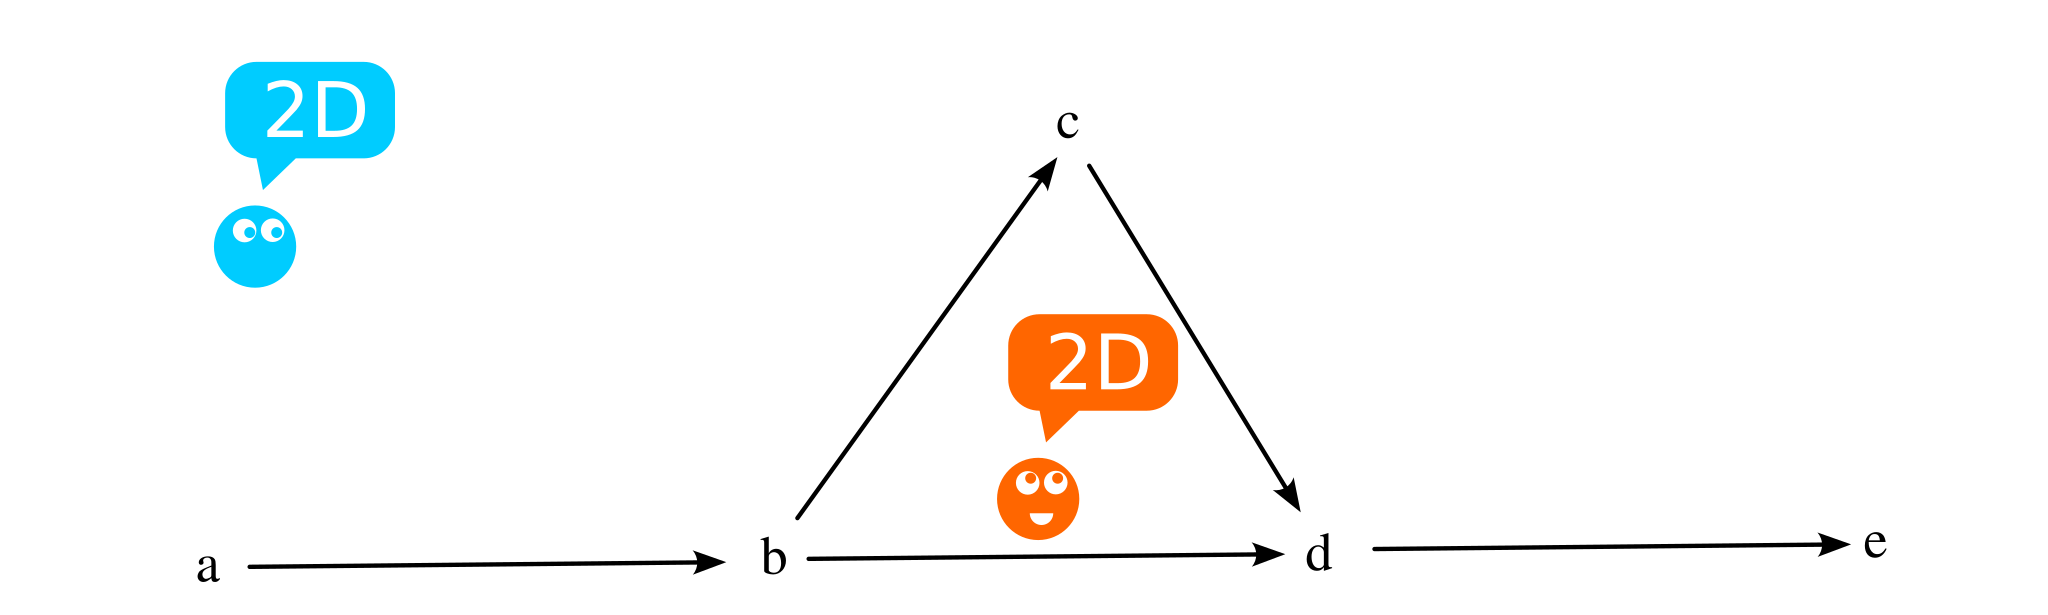
\includegraphics[width=\textwidth]{./2d-f1f2f3.png}
                \caption{Two-dimensional space}
                \label{fig:image}
            \end{figure}

            \item For the internal observer, there are two paths from \( f_{a,b} \) to \( f_{d,e} \)
            with different numbers of flumens (three and four). This is impossible in one-dimensional space,
            but is allowed in two-dimensional space, which the internal observer can recognize. The external observer perceives only
            the collection of flumens. They are not required to interpret the structure as
            two-dimensional, but they may choose to view it as such, based on the internal properties of the model.

            \item The two-dimensional space can be expanded by adding new flumens.

        \end{enumerate}


    \section{Spaces of Mixed Dimensions}
        \begin{enumerate}

            \item Let's add the flumens \( f_{e,f}=C(e,f) \) to the previous 
            set.

            \begin{figure}[H]
                \centering
                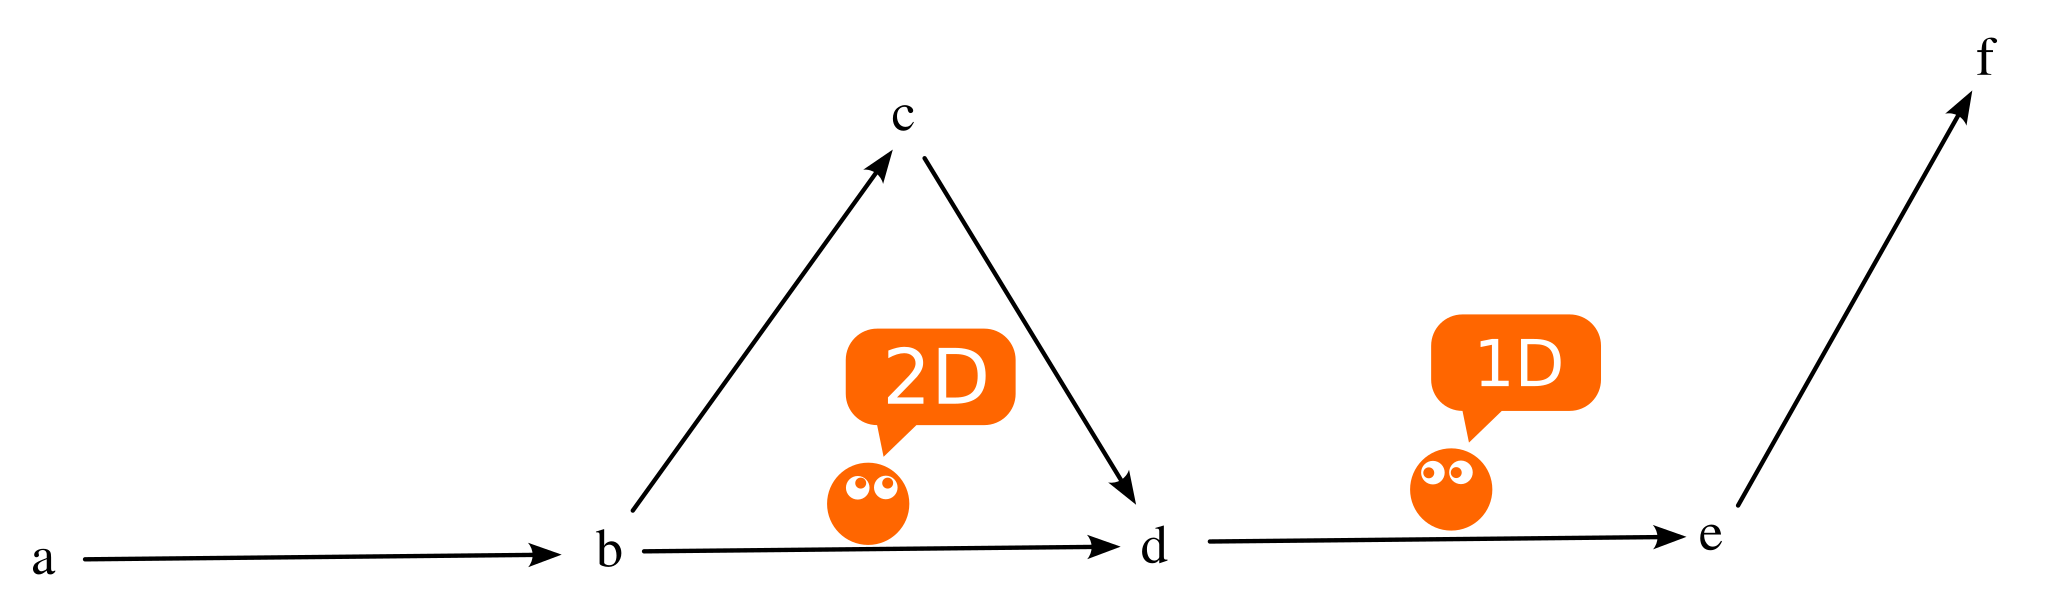
\includegraphics[width=\textwidth]{./2d-f1f2f3f4f5.png}
                \caption{One-dimensional and two-dimensional space}
                \label{fig:image}
            \end{figure}

            \item For the internal observer, the action within \( f_{b,c}, 
            f_{c,d}, f_{b,d} \) remains two-dimensional, but \( f_{d,e}, f_{e,f} 
            \) is perceived as one-dimensional, as there is a single path in 
            that section.

            \item This approach allows describing spaces with sections of 
            different dimensions, while maintaining the internal consistency of 
            the model.

        \end{enumerate}



    \section{Three-dimensional space and other dimensions}
        \begin{enumerate}
            \item Let's create the flumens as follows: \[ F =
            C[(a,b,c,b,a), (a,d,c,d,a), (a,c,a), (d,b,d)] \].

            \begin{figure}[H]
                \centering
                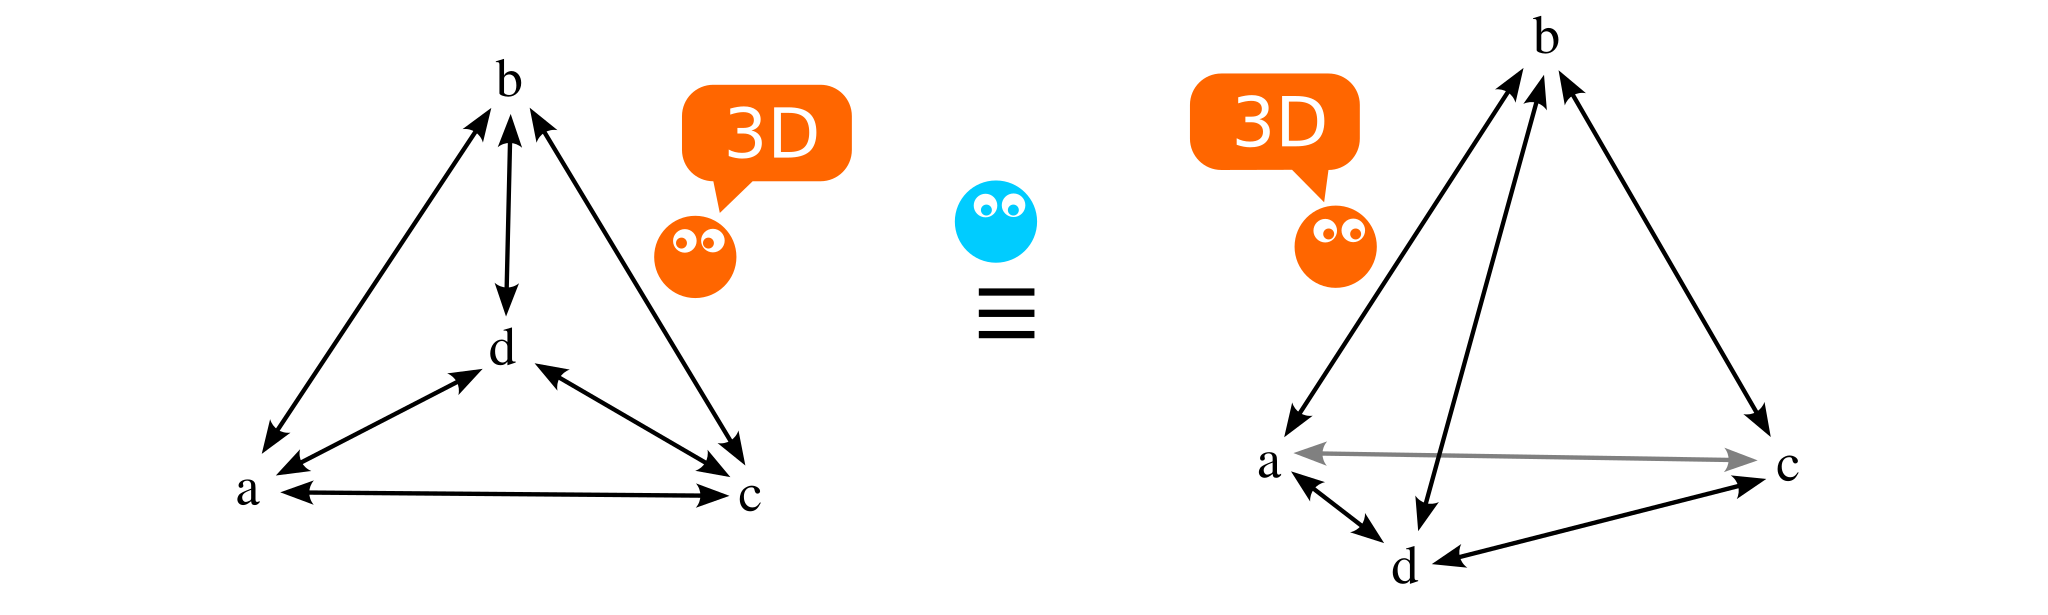
\includegraphics[width=\textwidth]{./3d-f1f2f3f4f5.png}
                \caption{Three-dimensional space}
                \label{fig:image}
            \end{figure}

            \item From the perspective of the External observer, the topology of 
            the two fragments shown above is identical. However, it is important 
            to remember that all the flumens are identical, and each will be 
            perceived by the Internal observer as a unit of space. When studying 
            the space, the Internal observer will be forced to recognize the 
            space as three-dimensional. Therefore, from their point of view, one 
            can speak of three-dimensional coordinates.

            \item For higher dimensions, such as four-dimensional space, the 
            same reasoning applies.

            \begin{figure}[H]
                \centering
                
\includegraphics[width=\textwidth]{./4d.png}
                \caption{Four-dimensional space}
                \label{fig:image}
            \end{figure}

        \end{enumerate}



    \section{Compact spaces}
        \begin{enumerate}

            \item Let’s create a two-dimensional space for the internal observer in a way different from before, for example: \( F[f_{a,b},f_{b,c},f_{c,a}] = C(a,b,c,a) \).

            \begin{figure}[H]
                \centering
                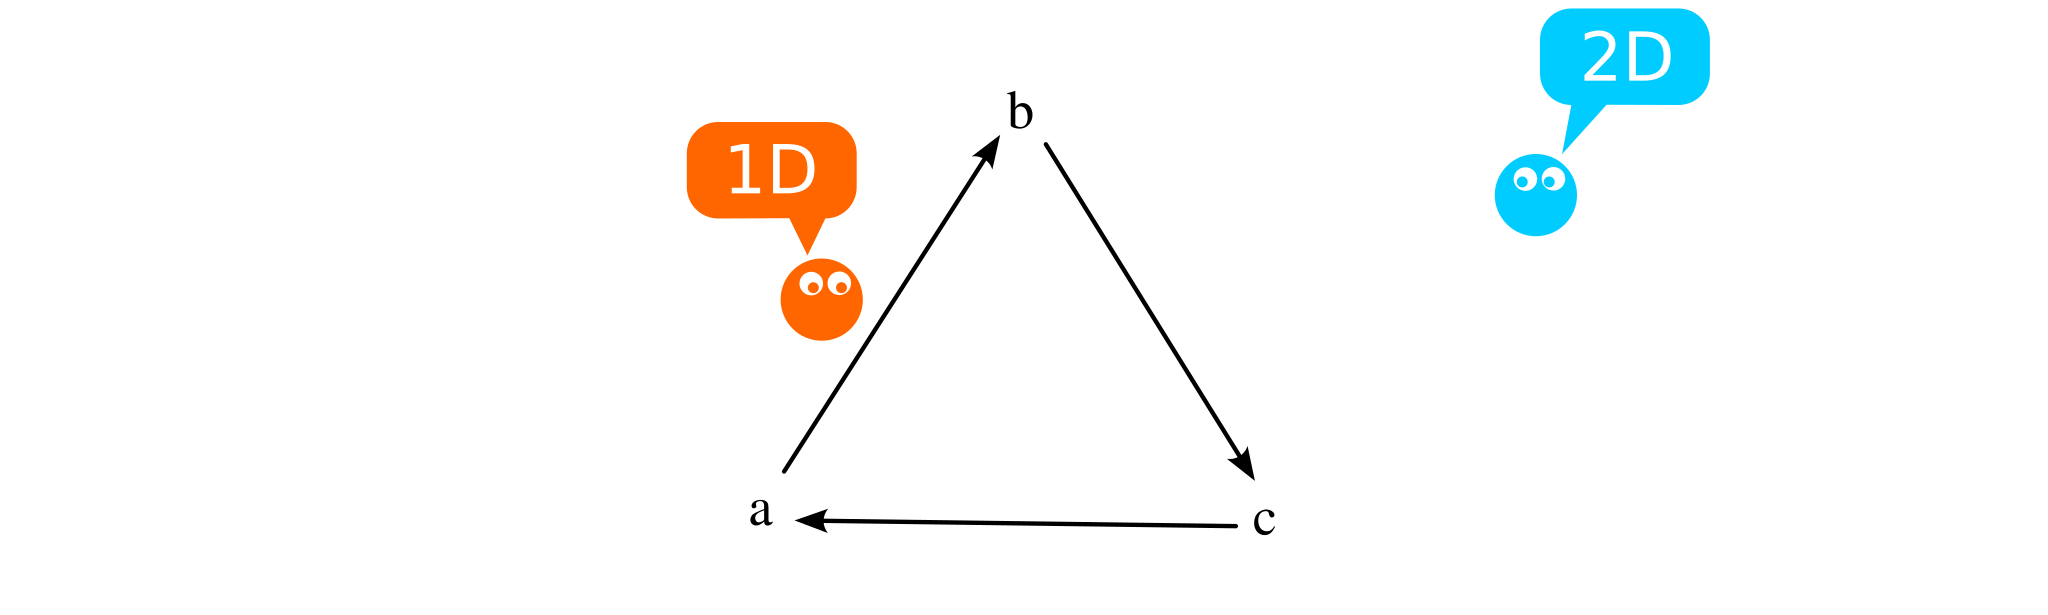
\includegraphics[width=\textwidth]{./2d-f1f2f3-loop.png}
                \caption{Compact one-way one-dimensional space}
                \label{fig:image}
            \end{figure}

            \item \(f_{a,b},f_{b,c},f_{c,a}\) form a closed seamless one-dimensional space for the Internal observer. The Internal observer can move infinitely in one direction.

            \item However, the External observer may interpret the movement from flumen to flumen as motion in a two-dimensional space.

            \item In a similar way, closed spaces of any dimension and configuration can be obtained, and it is possible to speak about their closure through higher dimensions.

        \end{enumerate}


    \section{"Artifacts of Fluemen"}

        By artifacts, we refer to the appearance of patterns that are absent in 
        the original data. The examples provided are just a small part of the 
        specific consequences of applying fluemen.

        \subsection{"Wormholes"}

            \begin{enumerate}

                \item Fluemen can form "wormholes" without the need for "curving 
                space," since at a fundamental level, space is not described. 
                Example: \[ F = C[(a,b,c,d,e,f),(b,c)] \]

                \begin{figure}[H]
                    \centering
                    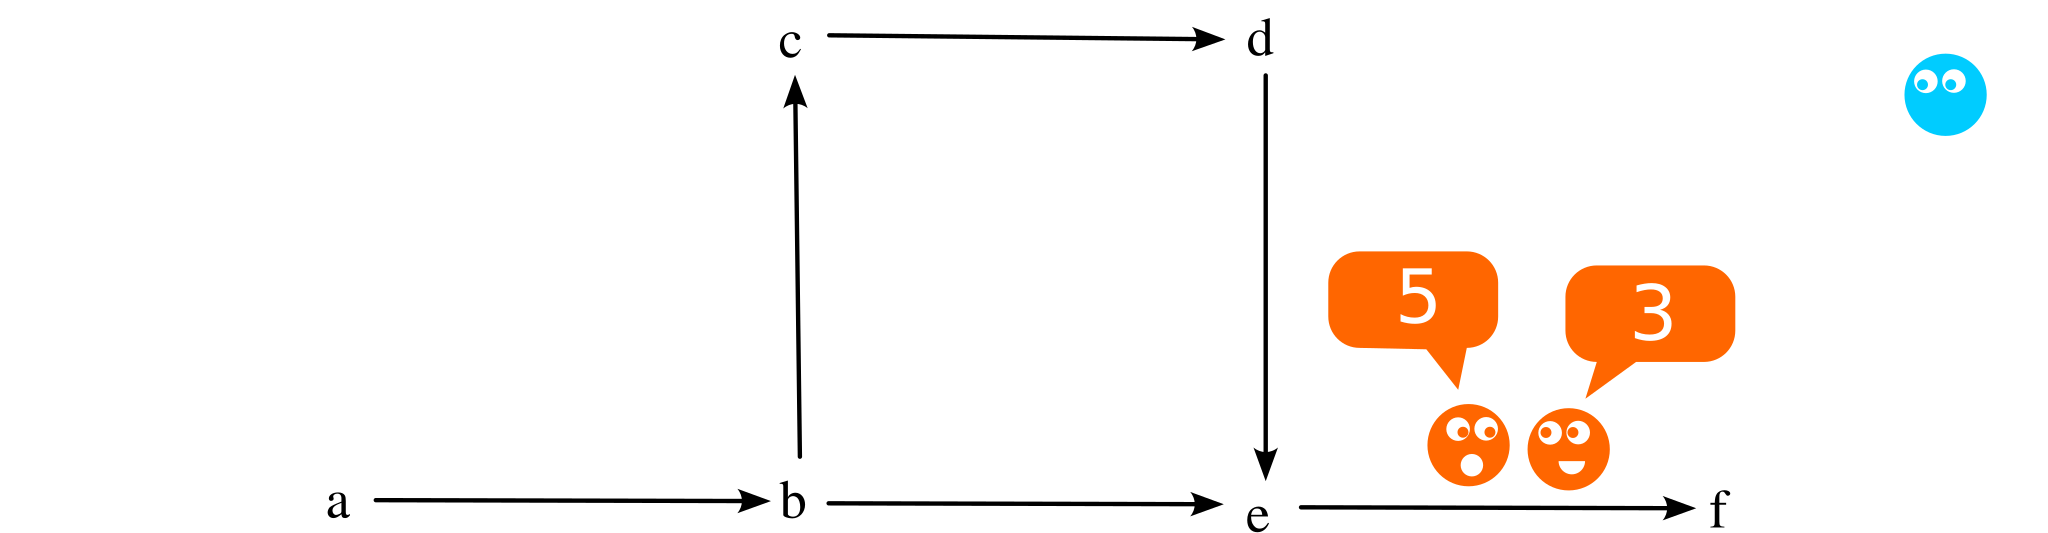
\includegraphics[width=\textwidth]{./wormhole.png}
                    \caption{"Wormhole illustration"}
                    \label{fig:image}
                \end{figure}

                \item The one-dimensional space, represented by fluemen 
                \(f_{a,b}, f_{b,c}, f_{c,d}, f_{d,e}, f_{e,f}\), is linear, 
                uniform, and continuous. Its length is 5 quanta.

                \item Fluemen \( f_{b,c} \) creates an alternative path from 
                \(f_{a,b}\) to \(f_{e,f}\) with a length of 3 quanta, which can 
                be interpreted as a "wormhole" from the perspective of the first 
                linear path.

                \item Such structures can be formed in spaces of any dimension, 
                allowing fluemen to model complex topologies.

            \end{enumerate}


        \subsection{"Parallel Spaces"}

            \begin{enumerate}

                \item Fluemen describe "parallel spaces," modeling identical or 
                partially different realities for observers. Example: \[ F = 
                C[(a,b,c,a,c,b,a), (d,e,f,d,f,e,d), (g,h,i,g)] \]

                \begin{figure}[H]
                    \centering
                    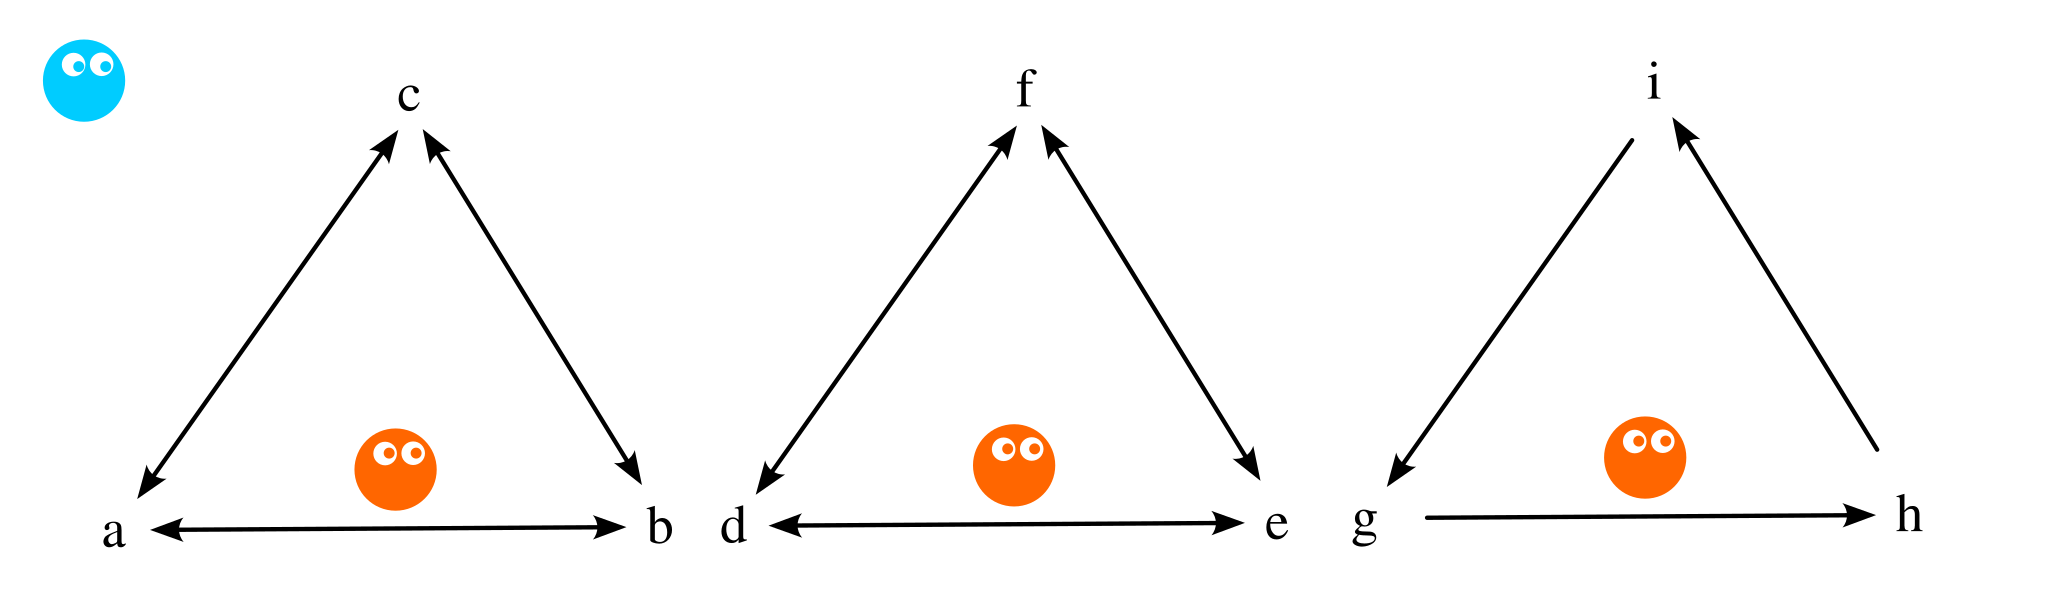
\includegraphics[width=\textwidth]{./parallel.png}
                    \caption{"Three parallel spaces"}
                    \label{fig:image}
                \end{figure}

                \item Observers cannot leave their subspaces and interact with 
                each other, while remaining in identical or nearly identical 
                conditions.

            \end{enumerate}



        \subsection{Domains}

            \begin{enumerate}

                \item The described spaces can be significantly more complex 
                than standard uniform ones, such as Cartesian spaces. For 
                example, the space of the Internal observer, consisting of 
                fluemen \(f_{d,h}, f_{h,d}, f_{h,i}, f_{i,h}, f_{i,d}, 
                f_{d,i}\), is one-dimensional and compact. However, it is part 
                of three domains \(abcd\), \(efgh\), and \(ijkl\), which lie 
                beyond the perception of the Internal observer. These domains 
                exceed the dimensionality of the observer's space and can 
                influence it.

                \begin{figure}[H]
                    \centering
                    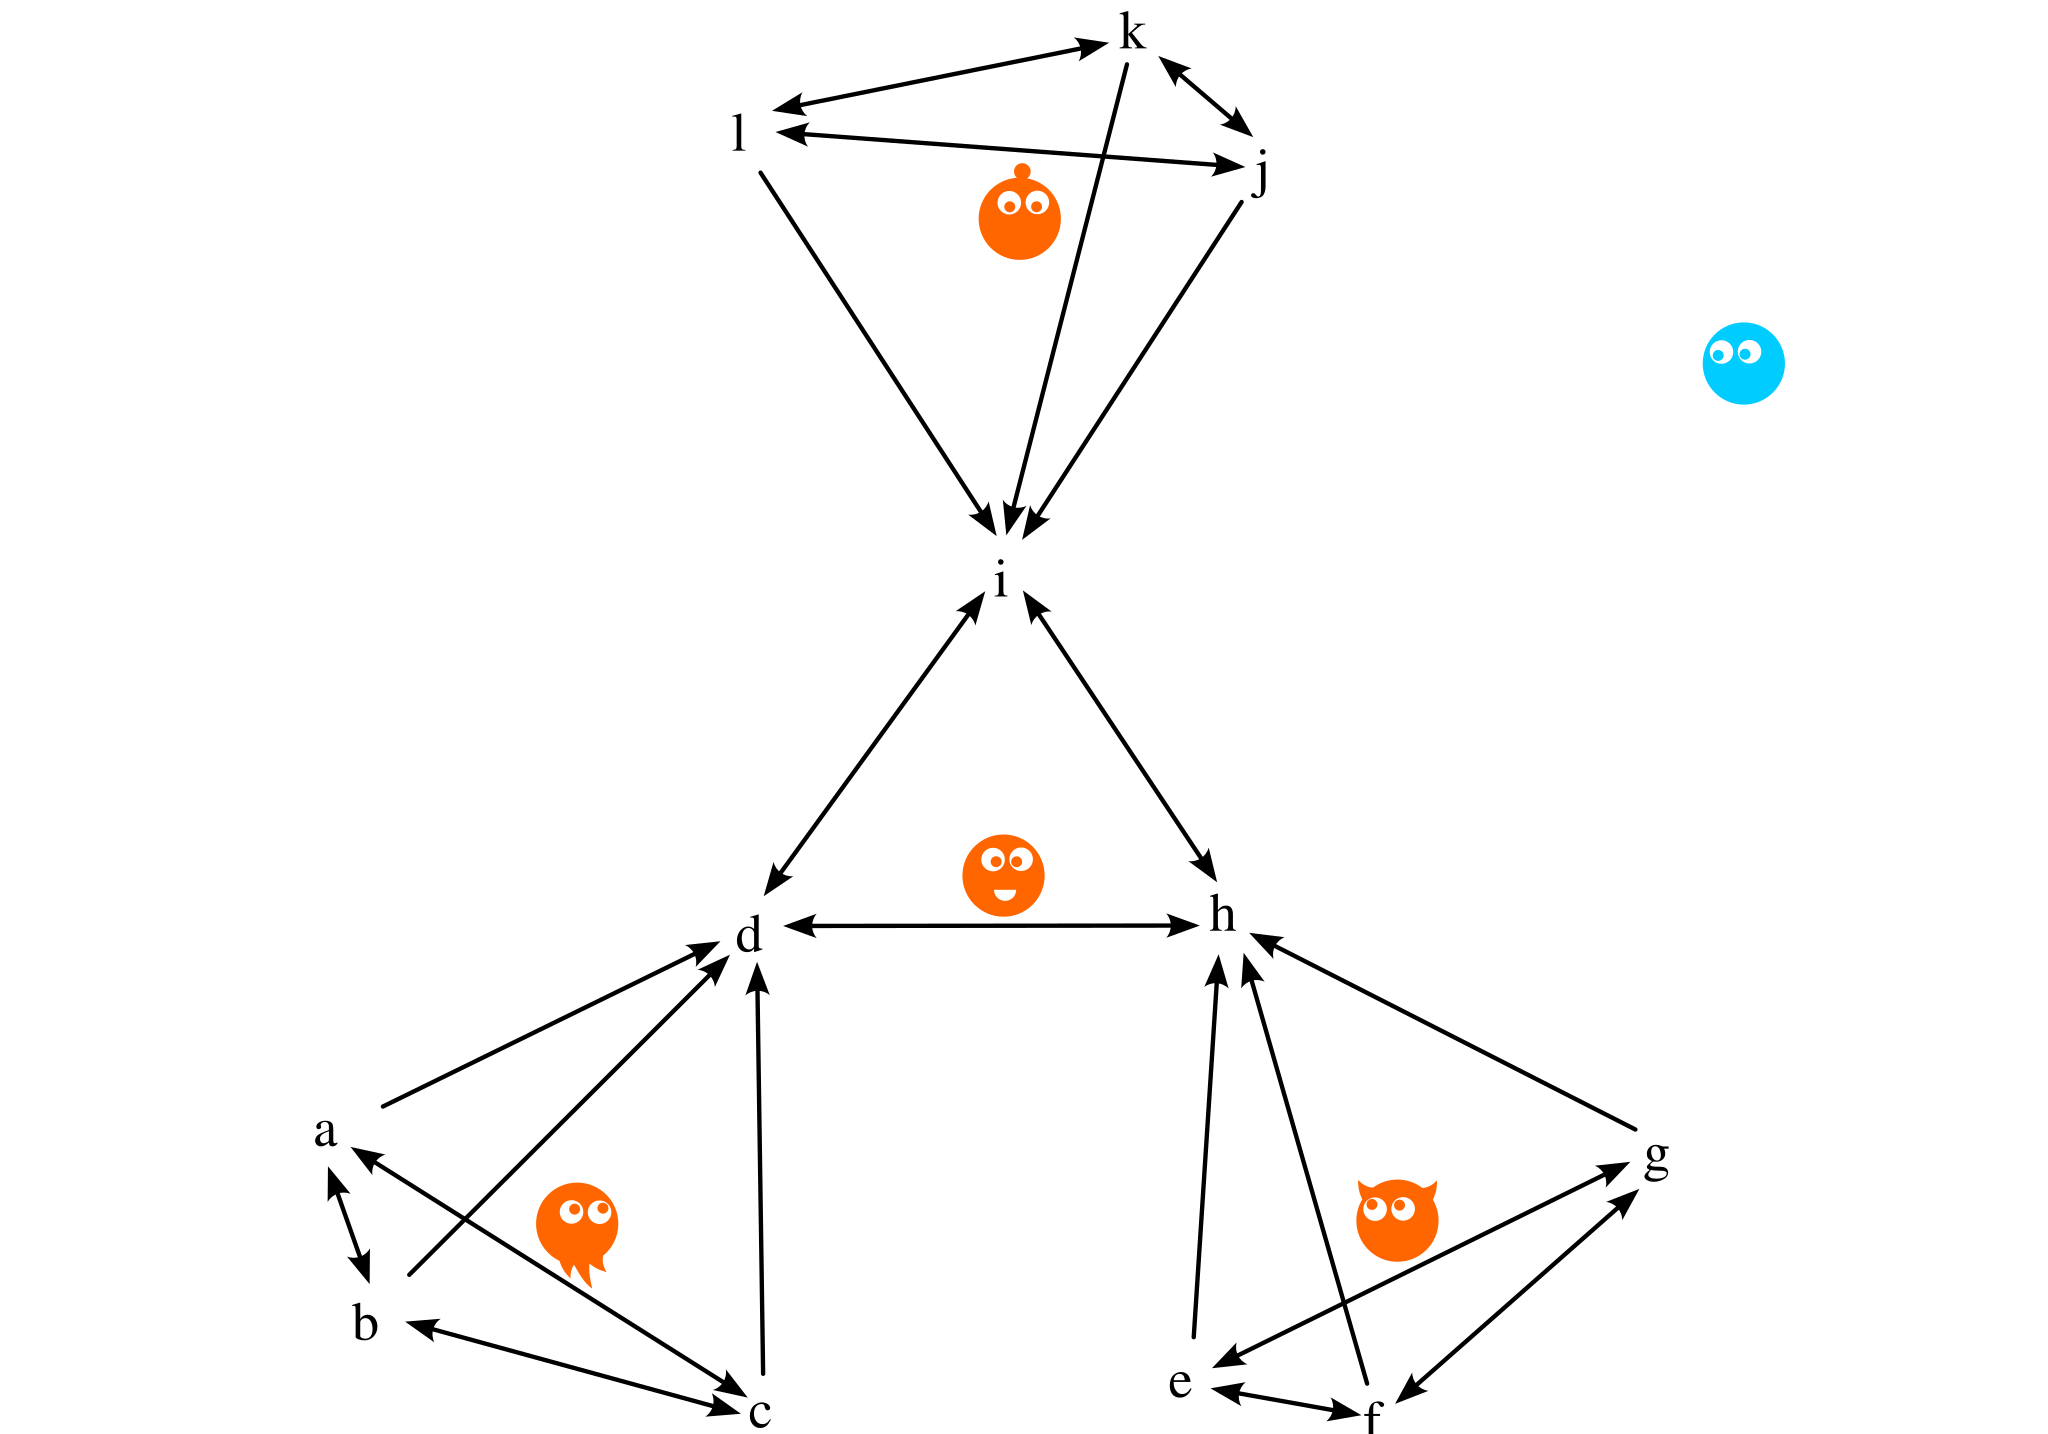
\includegraphics[width=\textwidth]{./domains.png}
                    \caption{Domains}
                    \label{fig:image}
                \end{figure}

            \end{enumerate}



    \section{Applicability of Fluemen}

        In addition to the examples and artifacts discussed, fluemen can be 
        useful for solving a number of other problems, such as:

        \begin{enumerate}

            \item Explaining the unidirectionality of time in multidimensional 
            spaces, which can be linked to symmetry principles in physics.

            \item Modeling the interconnection of multiple spaces of different 
            dimensions, topologies, and structures, for example, using domains 
            (\href{https://en.wikipedia.org/wiki/Brane}{branes}).

            \item Introducing the weight of fluemen allows its interpretation as 
            a deviation from the constant size of quanta, which in turn will 
            enable describing the dependence of the curvature of space on the 
            "energy" of its quanta in each individual region of space.

        \end{enumerate}


    \section{Summary}

        Fluemen offer a generalized method for modeling spaces with varying 
        dimensions, properties, and artifacts. Through a set of pairs of 
        natural numbers, they form the topology, configuration, and other 
        characteristics of these spaces.

    \begin{thebibliography}{9}

        \bibitem{wiki} Wiki
        \textit{Directed graph}
        \url{https://en.wikipedia.org/wiki/Directed_graph}

        \bibitem{hall1977} Hall, D. F. \textit{Introduction to Graph Theory}.
        Prentice-Hall, 1977.

        \bibitem{greene2000} Greene, B. \textit{The Elegant Universe:
        Superstrings, Hidden Dimensions, and the Quest to Understand the
        Ultimate Nature of Reality}. W.W. Norton \& Company, 2000.

    \end{thebibliography}

\end{document}
